\documentclass{report}
\title{Proposition de th\`ese}
\author{Yannick Hold-Geoffroy  \\
    Universit\'e laval  \\
    }

\date{\today}


\usepackage[utf8]{inputenc}
\usepackage{times}
\usepackage{amsmath}
\usepackage{amssymb}
\usepackage{cite}   % sort citation numbers automatically
\usepackage{url}
\usepackage{graphicx}
\usepackage{rotating}
%\usepackage{authblk}
% to control spacing in item lists
\usepackage{enumitem}
\usepackage[pagebackref=false,breaklinks=true,colorlinks,bookmarks=false]{hyperref}


% Hint: \title{what ever}, \author{who care} and \date{when ever} could stand 
% before or after the \begin{document} command 
% BUT the \maketitle command MUST come AFTER the \begin{document} command! 
\begin{document} 

\maketitle

% Commands
\newcommand{\boldomega}{\boldsymbol \omega} % bold omega
\newcommand{\boldmu}{\boldsymbol \mu} % bold omega
\newcommand{\bolddelta}{\boldsymbol \delta} % bold delta

\graphicspath{{figures/}}

%\begin{abstract}
%\end{abstract}


\chapter*{Symboles et notations}

\begin{table}[htbp]\caption{Symboles et notations}
\centering % to have the caption near the table
\begin{tabular}{r c p{10cm} }

\hline & & \\
$\langle \cdot, \cdot \rangle$      & $=$ & Produit scalaire \\
$\bold{x}$                          & $=$ & Vecteur \\
$X$                                 & $=$ & Matrice \\
$\omega$                            & $=$ & Angle \\
\hline
\end{tabular}
\label{tab:TableOfNotationForMyResearch}
\end{table}


\chapter{Introduction}

La numérisation du monde
Reconstruction 3d

\section{Contexte de la recherche}


\section{Vision future}

Utilisations: Jeux vidéos, préserver la culture, réalité augmentée, diffusion


\chapter{Description du projet}

La Stéréoscopie Photométrique (SP) est une technique permettant de récupérer la structure d'une scène à partir d'indices photométriques. Elle donne en sortie une carte de normale. Cette carte définie, pour chaque pixel de l'image, la normale de la surface correspondante dans la scène. Une fois la carte de normale obtenue, il est possible de l'intégrer afin d'obtenir un maillage 3d de la surface.

Pour fonctionner, la PS a besoin d'une séquence d'images en entrée.

\section{Stéréoscopie Photométrique}

Dans sa forme de base, la SP

\cite{Woodham1979}

\begin{equation}
\bold{b} = \rho L(\mathbf{\boldomega}) \langle \boldomega, {\bf n} \rangle \,,
\end{equation}

\begin{figure}
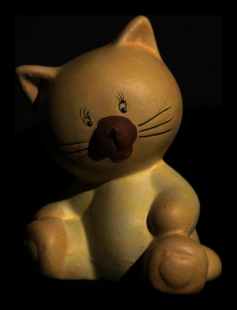
\includegraphics[width=.1\linewidth]{PS/cat_0.png}
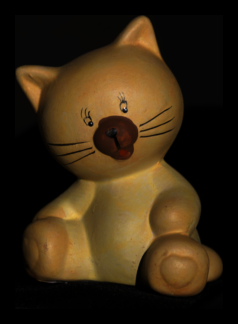
\includegraphics[width=.1\linewidth]{PS/cat_1.png}
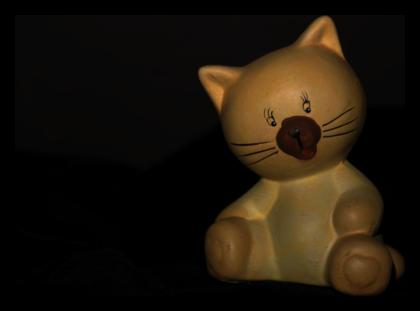
\includegraphics[width=.1\linewidth]{PS/cat_2.png}
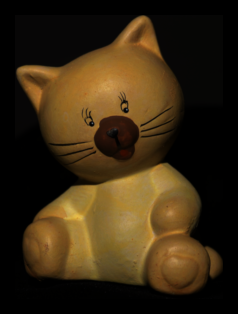
\includegraphics[width=.1\linewidth]{PS/cat_3.png}
\caption{Exemples d'images d'entrée}
\label{fig:fig}
\end{figure}


Force: 1 px par normale

\section{Contraintes extérieures}


\chapter{Revue de littérature}

\cite{Hold-Geoffroy-3DV15,Hold-Geoffroy-ICCP15}


\chapter{Solutions}

\section{Modèles d'illumination plus riche}

\begin{equation}
b_t = \frac{\rho}{\pi} \int_{\Omega_{\bf n}} L_t(\mathbf{\boldomega}) \langle \boldomega, {\bf n} \rangle d\omega \,,
\end{equation}

\section{Emploi d'autres astres que le soleil}

\section{Augmentation avec d'autres techniques}


\chapter{Échéancier}


\chapter{Conclusion}\label{conclusion}


{\small
%\bibliographystyle{ieee}
\bibliography{main}
}

\end{document}